\chapter{Results \& Discussion}

Recall that we split the practical work in two categories.  In this first instance, we tested the reviews projection learning algorithms on a common dataset and evaluation metrics as well as multiple embedding spaces.  We aimed at producing more statistical rigour than was presented in the original paper.  In the second set of experiments, we focused onto a particular algorithm, exploring it in some detail within the context of the shared task \citep{camacho2018semeval}.  The results of the conducted experiments are collated in this chapter.  

%\textbf{Should include a reiteration of the experiments, and their outcome.  Together with a description (discussion).  Preamble should include a reminder of the aims and objectives together with a list of experiments to achieve these.  Should include many charts and other visualization with appropriate descriptions}.  

\section{Hard-Clustering and Regularisation}
\subsection{Objectives}
\citeauthor{ustalov2017negative} proposed a set of regularistion terms, minimised alongside the \ac{MSE} objective function, designed to uphold the asymmetric nature of the hypernymy relation and discourage the model from projecting a query term close to its synonyms \citep{ustalov2017negative}.  We felt that the proposals were interesting but that the study's evidence of their efficacy was statistically weak.  Meanwhile, the chosen evaluation metrics - although sound - did not make it possible to compare the models with their projection learning peers \citep{yamane2016distributional, bernier2018crim}.  

We aimed to peruse of a standard set of metrics and employ a slightly-modified implementation provided by the SemEval-2018, Task 9 organisers \citep{camacho2018semeval}.  Moreover, we refactored the experimental setup such that produce a distribution of scores from a cross-validated dataset which allowed us to conduct a \textit{difference of means} hypothesis test.  Finally, we tested several embeddings feature spaces for observable differences in performance.

\subsection{Effect of Training Piecewise Projections}
\begin{figure}[ht!] 
  \centering
  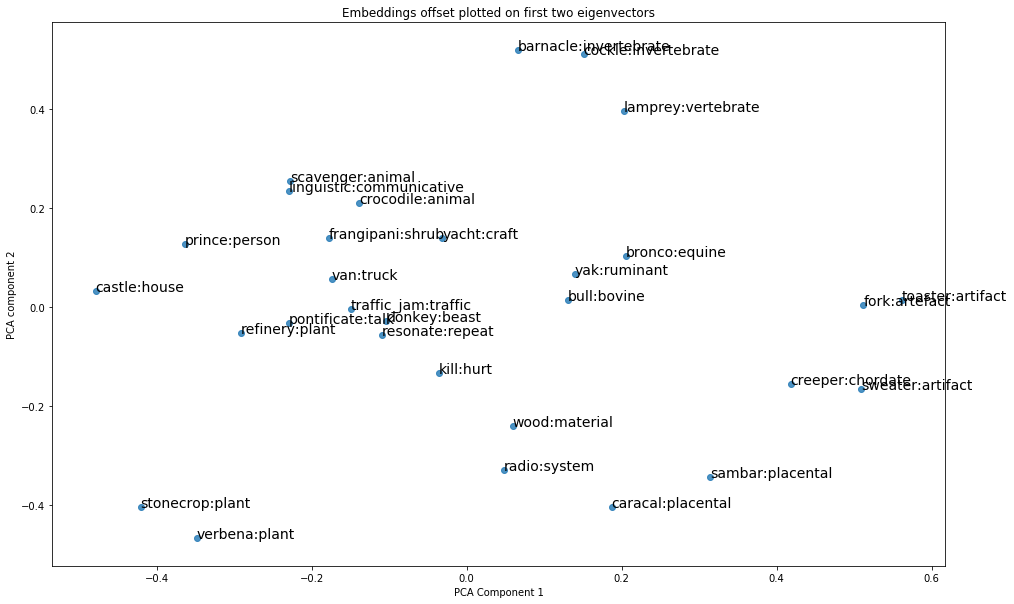
\includegraphics[width=1.\linewidth]{images/Sample_of_30_vector_offsets_PCA.png}
  \caption{Sample of 30 vector offsets projected on first two PCA components.}
  \label{fig:cluster_30_samp_pca}
\end{figure}
We evaluated single-cluster models that learned one transformation matrix for all the samples in the training dataset and multi-cluster models that first partition the word-pairs exclusively into a declared number of clusters.  We plotted 30 random vector offset samples projected on the first two eigenvectors of the word2vec embeddings space reduced by \ac{PCA}.  Despite that the PCA model only explains 15\% of the variance of the 30 samples, distinct clusters can be observed in Figure~\ref{fig:cluster_30_samp_pca}.  Plant vector (offsets) are occupying a cluster towards the bottom-left of the figure; \textit{equine}, \textit{ruminant} and \textit{bovine} vectors are clumped in a cluster at the centre of the plot whereas \textit{fork} and \textit{toaster} are grouped due to them being \textit{artefacts}.

\begin{figure}[ht!] 
  \centering
  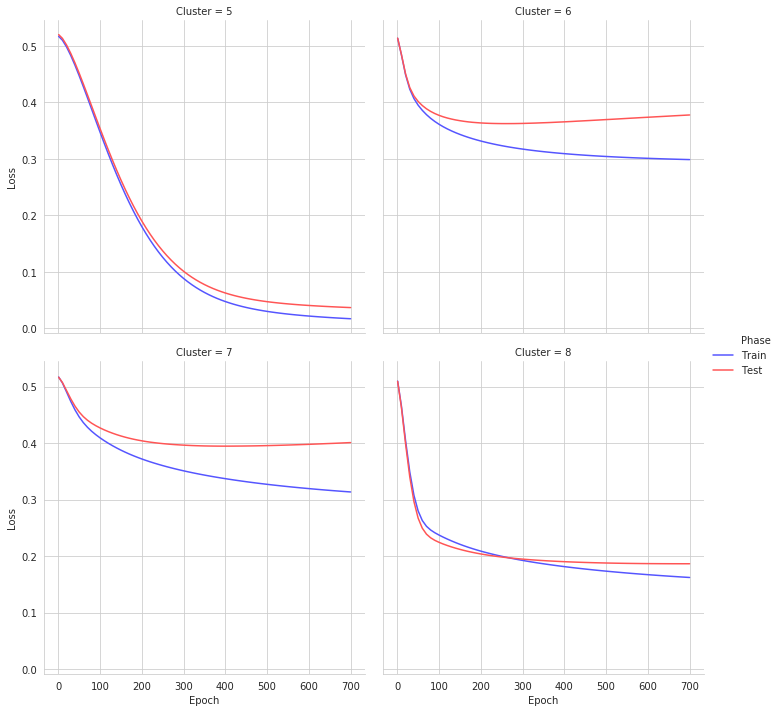
\includegraphics[width=1.\linewidth]{images/Train_losses_4_clusters_baseline_w2v.png}
  \caption{Train and validation loss on 4 data clusters (Baseline; word2vec).}
  \label{fig:train_test_loss_w2v}
\end{figure}

The training experience on the clusters differed.  We recorded the training and test loss returned when training a 10-cluster, baseline (i.e. no regularisation) model on an arbitrary training fold. This is the \citep{Fu2014} baseline as implemented in \citep{ustalov2017negative}.  We reproduced train and test losses for four clusters, chosen because of their idiosyncratic performance, in Figure~\ref{fig:train_test_loss_w2v}.

In some cases, such as \textit{cluster 5} (top-right panel), the cluster contained word-pairs featuring a distinctive linear relation between hyponym and hypernym vectors, a fact which was captured by the model.  The test loss mirrors the training loss almost perfectly which suggests that the members of the 5$^{th}$ test cluster belong to the same semantic family of the word-pairs in the training cluster.  The 6$^{th}$ and 7$^{th}$ cluster do not fare as well: over-fit is manifested at the 150-200 epoch mark and the end-of-training loss is markedly higher than what was observed in the 5$^{th}$ cluster.  A balanced performance was delivered by the 8$^{th}$ cluster: no over-fit and a reasonable end-of-training loss.

\subsection{Baseline against Regularised Model Results}
\begin{figure}[ht!] 
  \centering
  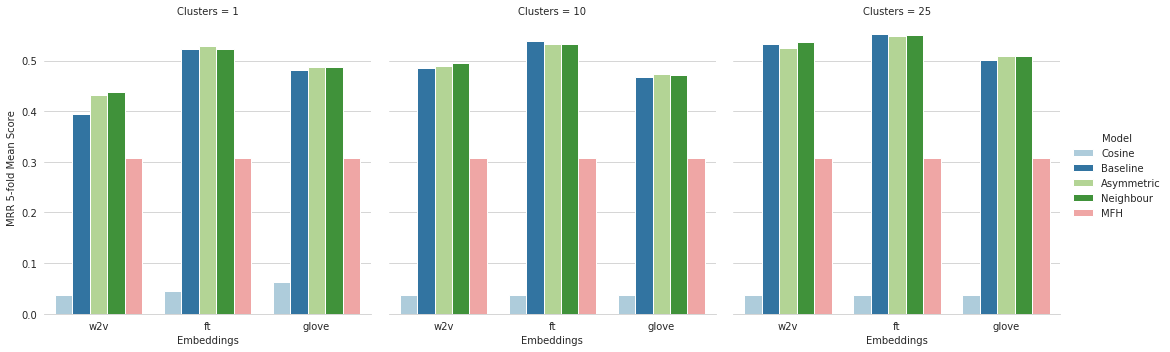
\includegraphics[width=1.\linewidth]{images/MRR_5-fold_results_models_baselines_embeddings.png}
  \caption{Mean MRR cross-validated results when evaluated on different cluster sizes, baselines, models and embeddings.}
  \label{fig:MRR_models_baselines}
\end{figure}

\begin{figure}[ht!] 
  \centering
  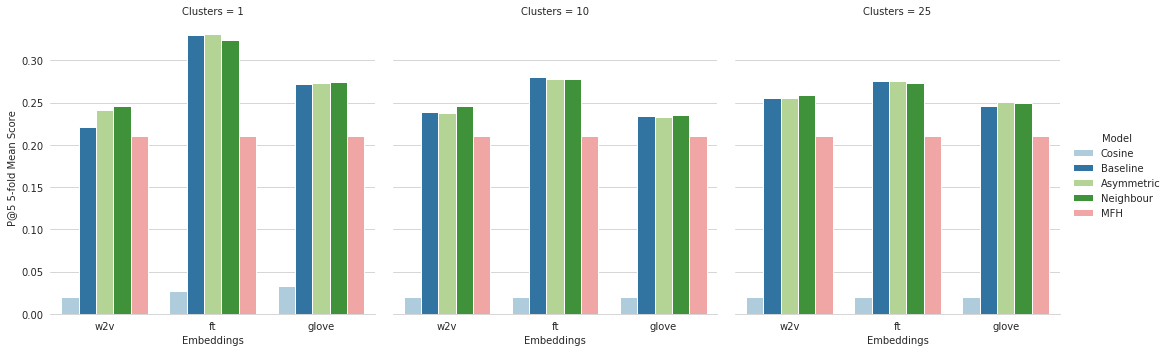
\includegraphics[width=1.\linewidth]{images/PAt5_5-fold_results_models_baselines_embeddings.png}
  \caption{Mean P$@5$ cross-validated results when evaluated on different cluster sizes, baselines, models and embeddings.}
  \label{fig:pat5_models_baselines}
\end{figure}

We measured the models' performance on the basis of 5 metrics: \ac{MRR}, \ac{MAP}, and P$@k$ where $k \in \{1, 5, 10\}$.  We report MRR, MAP results since they were largely found to be uncorrelated according to the Spearman rank-order correlation test. \footnote{The only exceptions were the word2vec MAP, MRR results which were correlated with a score of 0.988 at 99\% confidence.}   We also report P$@5$ results for completeness but omit P$@1$ and P$@10$ due to space considerations.  P$@k$ results are positively correlated with \ac{MAP} according to the Spearman rank-order correlation.

According to our cross-validated experiments on randomly-split datasets, the regularised models exert only a slight influence on the results, except for those observed on the single cluster model trained on word2vec embeddings features.  MRR scores are plotted in Figure~\ref{fig:MRR_models_baselines}.  MRR rewards models for which the first discovered, correct hypernym per term is ranked highly.  \citeauthor{ustalov2017negative}'s modifications slightly harm the models in the fastText 10 and 25 cluster scenarios.  The most-pronounced effect of regularisation was observed with the single-cluster model trained on word2vec embeddings features.  MRR improved by 9.5\% and 11.2\%  with the asymmetric and neighbour regularisation models respectively.  P$@5$ results are plotted in Figure~\ref{fig:pat5_models_baselines}.  Similar to the MRR results, regularisation has left the largest impact on the single-cluster model trained on word2vec features.
\begin{table*}\centering
\begin{tabular}{@{}lrrrrrrrrrr@{}}\toprule
& \multicolumn{2}{c}{\textit{Baseline Sample}} & \multicolumn{4}{c}{\textit{Asymmetric Reg. Sample}} &
\multicolumn{4}{c}{\textit{Neighbour Reg. Sample}}\\
\cmidrule{2-11}
& $\bar{x}$ & $\pm\sigma_{\bar{x}}$ & $\bar{x}$ & $\pm\sigma_{\bar{x}}$ & $t$ & $p$ & 
$\bar{x}$ & $\pm\sigma_{\bar{x}}$ & $t$ & $p$ \\ \midrule
\textit{w2v}\\
\textit{1} & 0.227 & 0.016 & 0.249 & 0.010 & \textcolor{blue}{-2.601} & \textcolor{magenta}{\textbf{0.030}} & 0.253 & 0.011 & \textcolor{blue}{-3.032} & \textcolor{magenta}{\textbf{0.019}}\\
\textit{10} & 0.254 & 0.011 & 0.253 & 0.020 & \textcolor{blue}{0.080} & \textcolor{magenta}{0.470} & 0.261 & 0.011 & \textcolor{blue}{-0.674} & \textcolor{magenta}{0.269}\\
\textit{25} & 0.275 & 0.008 & 0.273 & 0.016 & \textcolor{blue}{0.249} & \textcolor{magenta}{0.408} & 0.278 & 0.011 & \textcolor{blue}{-0.390} & \textcolor{magenta}{0.358}\\
\cmidrule(lr){2-11}
\textit{GloVe}\\
\textit{1} & 0.284 & 0.015 & 0.285 & 0.019 & \textcolor{blue}{-0.084} & \textcolor{magenta}{0.468} & 0.285 & 0.014 & \textcolor{blue}{-0.151} & \textcolor{magenta}{0.443}\\
\textit{10} & 0.248 & 0.019 & 0.248 & 0.034 & \textcolor{blue}{-0.005} & \textcolor{magenta}{0.498} & 0.250 & 0.020 & \textcolor{blue}{-0.093} & \textcolor{magenta}{0.465}\\
\textit{25} & 0.262 & 0.013 & 0.268 & 0.017 & \textcolor{blue}{-0.600} & \textcolor{magenta}{0.290} & 0.267 & 0.012 & \textcolor{blue}{-0.443} & \textcolor{magenta}{0.340}\\
\cmidrule(lr){2-11}
\textit{fastT}\\
\textit{1} & \textbf{0.339} & 0.019 & \textbf{0.341} & 0.014 & \textcolor{blue}{-0.211} & \textcolor{magenta}{0.422} & \textbf{0.334} & 0.015 & \textcolor{blue}{0.462} & \textcolor{magenta}{0.334}\\
\textit{10} & \textbf{0.295} & 0.024 & \textbf{0.291} & 0.010 & \textcolor{blue}{0.271} & \textcolor{magenta}{0.400} & \textbf{0.292} & 0.021 & \textcolor{blue}{0.215} & \textcolor{magenta}{0.420}\\
\textit{25} & \textbf{0.293} & 0.009 & \textbf{0.293} & 0.020 & \textcolor{blue}{0.005} & \textcolor{magenta}{0.498} & \textbf{0.292} & 0.012 & \textcolor{blue}{0.154} & \textcolor{magenta}{0.443}\\
\bottomrule
\end{tabular}
\caption{Statistical analyses of regularised \ac{MAP} improvements over baselines in multi-cluster, multi-embeddings settings.}\label{tab:t_test_regularised}
\end{table*}
We ran statistical significant tests on our experiment results and plot the values in Table~\ref{tab:t_test_regularised}.  In this table we are comparing the performance of the various regularised models against a non-na\"ve baseline, while controlling for embeddings and cluster size.  The $t-$values (in blue) are computed according to the Welch t-test and are negative if the mean of the baseline is less than the mean of the regularised model, and positive if the mean of the baseline is larger than the mean of the regularised model.  The $p-$values are in pink and reflect a left-tailed test if the $t-$value is negative and a right-tailed test if it is positive.  The objective is to assess whether the baseline mean is significantly smaller or significantly greater than the mean MAP of the regularised models depending on the observed results.  We marked the overall best \ac{MAP} results in bold. Significant p-values at 95\% confidence are also set in bold.

\subsection{Single Cluster against Multi-Cluster Model Results}
We measured statistical significance at 95\% confidence for difference of means in \ac{MAP} obtained when training a single cluster model against several clusters, controlling for model type and embeddings.  

Increasing the cluster size seems to have a favourable effect on the word2vec models in most cases, particularly when training a 25-cluster baseline model for which a 21.4\% \ac{MAP} score improvement over the single-cluster variant was registered.  Less pronounced, but nonetheless significant, improvements were recorded on the regularised models while a 10-cluster model had a moderate effect on \ac{MAP} where a significantly better result was only noted with the baseline model.  

Increasing cluster size had a detrimental effect on models trained on GloVe embedddings.  Specifically, the \ac{MAP} scores dipped significantly for the baseline and neighbour regularisation models while the asymmetric model was insignificantly worse.  The deterioration was not as conspicuous between the single cluster and 25-cluster models, although the performance of the latter suffered compared to the simpler model.  

Multi-clusters harmed the fastTest models even more.  All single-cluster models were significantly better-performing than the 10-cluster and 25-cluster variants, whereby every multi-cluster model suffered an average decrease of 13.4\% of its corresponding single-cluster \ac{MAP} score.

\subsection{Embeddings Effect} \label{ustalov_embeddings}
We observed the overall best \ac{MAP} result with a single-cluster model trained on fastText embeddings with asymmetric regularisation (0.341) which was significantly better - at 95\% confidence - than both the Fiword2vec and GloVe models, controlling for cluster-size and model type.  Moreover, fastText \ac{MAP} results were the best in every other category and significantly better than those returned in the equivalent word2vec-based experiments, with the exception of the 25-cluster regularised models in which the results, although better, were not significantly so at 95\% confidence.

GloVe embeddings' \ac{MAP} scores were significantly better (95\% confidence) than the corresponding word2vec models only in the single-cluster experiments.  In the rest of the scenarios, GloVe features yielded the worst results, although not significantly worse than the word2vec scores. 

\subsection{Naïve Baselines}
We also note from Figures~\ref{fig:MRR_models_baselines},~\ref{fig:pat5_models_baselines} that all trained models have an edge on the na\"ve baselines.  The \ac{MFH} yields better results than cosine similarity across the base, but is bettered by even the worst-performing trained model in all scenarios.

%% Results are interpreted in the evaluation.  Significant is only observed in one particular scenario - w2v; single cluster.
\subsection{Lexically-Split Experiment Results}
\begin{figure}[ht!] 
  \centering
  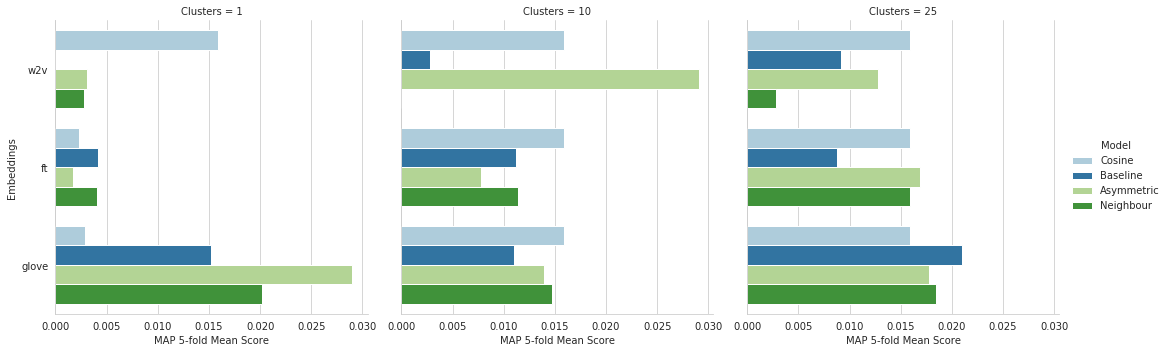
\includegraphics[width=1.\linewidth]{images/MAP_lexical_split_results_models_baseline_embeddings.png}
  \caption{\ac{MAP} results obtained on lexically-split dataset with baseline and regularised models across various embeddings.}
  \label{fig:lexsplit_ustalov_map}
\end{figure}
In the lexically-split dataset, we ensured that a word in the hypernym slot of a word-pair either features in training set or the test set but not in both.  The \ac{MAP} results are reproduced in Figure~\ref{fig:lexsplit_ustalov_map}.  The results were much lower throughout compared to the results obtained by models trained on randomly-split data.  Nine configurations achieved scores that were very close to 0.  fastText features scored poor results with the single-cluster models, in stark contrast to what we observed in section \ref{ustalov_embeddings}.  On the other hand, the single-cluster model with asymmetric regularisation trained on GloVe features, achieved the best \ac{MAP} result (0.029).  This score was tied with the 10-cluster word2vec model also including the asymmetric regularisation term.  Notwithstanding, there is configuration which is discernibly better than the other.  Similar to other work \citep{shwartz2017siege}, the cosine unsupervised metric demonstrated robustness in the face of lexical split, returning results nominally worse than those returned in the random data split experiments.

We should also note that the SemEval-2018 Task 9 evaluation code takes into consideration the number of gold hypernyms per test term, ignoring predictions which are ranked in a position greater than the length of the gold hypernym list.  The lexical split decreased the dataset substantially such that each test term is associated with only a single gold hypernym.  Thus, predicted hypernyms ranked second and lower are discarded by the evaluation code outright and never evaluated for correctness.  

Lastly, the \ac{MFH} baseline results were deliberately excluded since they do not apply to a lexically-split dataset context.
%Mention that MFH baseline is indifferent to the embeddings since it uses simple lexical frequency rather feature vectors

